The focus is on the security aspects of autonomous on-roar motor vehicles,
in particular the cybersecurity threats, standards, and industry practices used to secure these systems.
The focus will be on the current state of the art of the communication main technologies and sensors,
analyzing the attack surface, main vulnerabilities and possible countermeasures to take.
Starting from a brief of history of AVs and introducing an overview of the architecture, and then focusing on the main sensors and communication technologies used in AVs.
Every section will pay attention mostly on the cybersecurity aspects, so some other aspects can be omitted.
Through this analysis, the review aims to respond to the research question currently in the methodology section.
This review will not cover the ethical implications or the differences between human-driven and autonomous vehicles in terms of accidents and fatalities.
Moreover, the review will not cover the security of other autonomous systems
but focuses only on the on-road motor vehicles and its main parts.

\subsection{Structure of the Survey}\label{subsec:structure-of-the-survey}

\subsection{Historical roots}\label{subsec:historical-roots}

The development of autonomous vehicles is a significant milestone in the evolution of intelligent transport systems.
It is important to start with some historical context to understand the current state of autonomous vehicles and then,
the security implications.

Vehicle automation has roots dating back to 1918 \cite{pendleton2017perception} ,
with General Motors showcasing the first concept of an automated vehicle in 1939 \cite{shladover2017connected} .
Initial R\&D efforts were led by General Motors and the Radio Corporation of America Sarnoff Laboratory in the 1950s.
From 1964 to 2003, various government and academic initiatives in the US, Europe,
and Japan focused on automated buses, truck platoons, and advanced driving systems
\cite{shladover2017connected} .
A significant boost came from DARPA’s Grand Challenges Program in the 2000s \cite{darpa_grand_challenges_book},
where AVs first navigated desert terrains in 2005 and urban roads by 2007 \cite{pendleton2017perception, shladover2017connected}

Since then, researchers have rapidly progressed in academia and industry.
Volvo, Tesla, Audi, BMW,
Mercedes-Benz and Nissan are some of the major car manufacturers that have invested in AV technology \cite{faisal2019understanding}.

\begin{figure}[!htb]
    \centering
    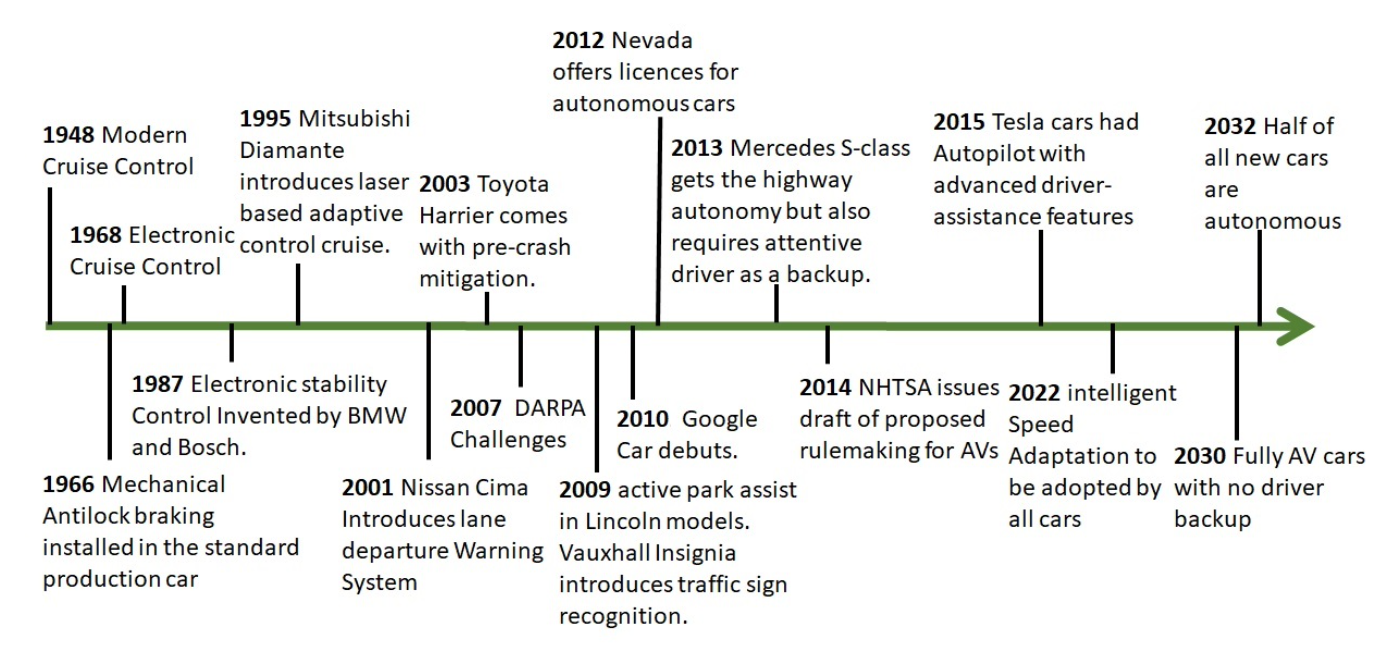
\includegraphics[width=0.7\linewidth]{figures/history}
    \caption{Historical timeline of autonomous vehicles.}
    \footnotesize{From \cite{ahangar2021survey} }
    \label{fig:history}
\end{figure}

\subsection{Autonomous Vehicles}\label{subsec:autonomous-vehicles}

The introduction on the market of autonomous vehicle brings to a revolutionary change in the automotive sector.
Many sectors can be influenced by the introduction of these vehicles, obviously not only the automotive one but also the legal and the urban planing are only examples of the sectors that can be influenced by the introduction of these vehicles.
This type of vehicle brings us to a new era of mobility, where transportation systems become intelligent and connected.

This major challenge, as often happens during times of innovation, has brought both advantages and drawbacks in terms of security.
By this, I mean that the real driving force behind this innovation has been the convenience and socially beneficial aspects that have led to the rapid growth of the sector.
However, as is often the case in such situations, some fundamental details get overlooked—it's a natural consequence.
In this case, the concept of cybersecurity by design has been neglected \cite{sec-by-design}, and, much like the early days of the web, efforts are now being made to address it.

Also in terms of communication, a lot of innovations have been made because of the introduction of these vehicles.
To improve functionalities, infotainment, safety, comfort and a lot of other aspects, vehicles require a lot of communication between them and the infrastructure.
The shift from isolated and static systems to dynamic and interconnected systems increases the complexity of security issues, particularly in terms of adaptability, dynamism, and self-awareness \cite{connected_vehicles_security_2023, bouchouia2023survey} .

For instance, vehicles relying on open software protocols and connecting with in-vehicle electric infrastructures play a vital role in strengthening their security framework.
With the integration of advanced sensor platforms, these vehicles essentially evolve into highly sophisticated set of technologies influencing each other expanding the attack surface \cite{sec-by-design} .


\subsubsection{Levels of Automation}\label{subsubsec:levels-of-automation}
The level of driving automation is determined by the specific roles assigned to both the driving automation system feature and the human user in performing the dynamic driving task (DDT) and DDT fallback. \cite{sae_j3016_2021}
The manufacturer of the automation system defines the requirements, operational design domain (ODD), and operating characteristics of the feature, including its level of automation.
Additionally, the manufacturer outlines how the feature should be properly used, ensuring that its capabilities and limitations are clearly understood and followed during operation.
The Society of Automotive Engineers (SAE) has defined six levels of driving automation, ranging from no automation (Level 0) to full automation (Level 5) \cite{sae_j3016_2021}.

\begin{enumerate}
    \item \textbf{Level 0 (No Automation):} The human driver is responsible for all aspects of the dynamic driving task.
    \item \textbf{Level 1 (Driver Assistance):} The vehicle assists the driver with specific tasks, such as steering or acceleration.
    \item \textbf{Level 2 (Partial Automation):} The vehicle can control both steering and acceleration/deceleration simultaneously under certain conditions, but the driver must remain engaged and monitor the environment.
    \item \textbf{Level 3 (Conditional Automation):} The vehicle can perform all aspects of the DDT under certain conditions like in traffic jams or highway driving, but the driver must be ready to take over when prompted.
    \item \textbf{Level 4 (High Automation):} The user (become passenger) does not need to supervise the Automated driving system (ADS) or be receptive to a request to intervene while the
    ADS is engaged, restricted to some conditions (e.g. Google's Self-Driving Car \cite{teoh2017rage}).
    \item \textbf{Level 5 (Full Automation):} The vehicle can perform all aspects of the DDT under all conditions without human intervention.
\end{enumerate}

\begin{table}[ht]
    \centering
    \begin{tabular}{|c|l|}
        \hline
        \textbf{Acronym} & \textbf{Definition} \\ \hline
        ADS & Automated Driving System \\ \hline
        DDT & Dynamic Driving Task \\ \hline
        ODD & Operational Design Domain \\ \hline
        OEDR & Object and Event Detection and Response \\ \hline
    \end{tabular}
    \caption{Definitions of Key Acronyms in Automated Driving}
    \label{tab:acronyms}
\end{table}

Levels 0–2 are generally classified as driver-assisted systems, while Levels 3 and 4 are considered semi-automated, and Level 5 represents full autonomy.

\subsection{Overview of AVs Architecture}\label{subsec:overview-on-avs-architecture}

This section provides an high-level overview of thee autonomous vehicles (AVs) architecture and the key parts that enable their operation.
Moreover, an alternative architecture proposed in \cite{2023survey} will be briefly discussed.
The architecture of AVs is designed to integrate various hardware and software components that work together to perceive the environment, make decisions, and control the vehicle.

\cite{architecture}

\begin{figure}[!htb]
    \centering
    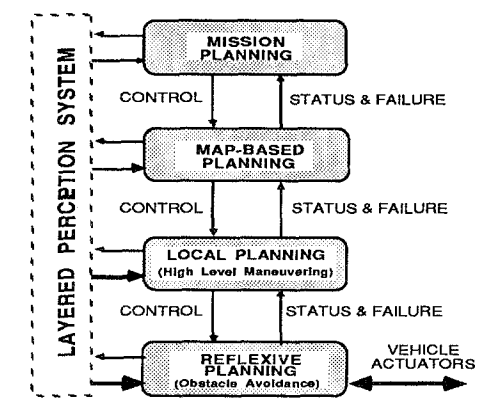
\includegraphics[width=0.7\linewidth]{figures/state-architecture}
    \caption{Hierarchical architecture of autonomous vehicles control.}
    \footnotesize{From \cite{architecture} }
    \label{fig:architecture}
\end{figure}

The current architecture presented in \ref{fig:architecture} is composed of layers of hardware and software that interact to enable the vehicle to operate autonomously.
In its simplest form, the architecture consists of four main layers: perception, decision and planning, control and reflexive.
Each layer is responsible for a specific aspect of the AV's operation, from sensing the environment to executing driving maneuvers reflexively \cite{architecture} .

\begin{enumerate}
    \item \textbf{Perception}: This stage involves sensing the AV's surroundings using sensors that will be presented successively in SECTION. The information is processed by recognition modules, such as adaptive detection and recognition frameworks, control systems, lane departure warning systems, traffic sign recognition, obstacle recognition, and vehicle positioning modules.
    The processed data is then sent to the decision and planning stage.
    \item \textbf{Decision and Planning}: Using the data from the perception stage, this stage plans and controls the AV's motion and behavior.
    It handles tasks like path planning, action prediction, and obstacle avoidance based on real-time maps, traffic data, user inputs, and past information.
    It may also include a data log module for error tracking and future reference.
    \item \textbf{Control}: The control module receives instructions from the decision and planning stage and manages the physical functions of the AV, such as steering, braking, and acceleration.
    \item \textbf{Reflexive}: This final stage interfaces with the mechanical components like the motors for the accelerator, brake, steering wheel, and gear.
    These components are controlled by the signals from the control module to execute the AV’s movements.
\end{enumerate}

The proposed and secured architecture extends the just presented one providing four new layer: monitoring, analysis, decision-making, and visualization.
Any services, processes, and communication are monitored by the agents and analyzed by the process controllers.
A set of decision controllers act on the information from the process controllers.
The decisions are archived in a black box, while the analysis, reporting, and visualization layers are accessible both within the vehicle and through an external Virtual Security Operations Center (VSOC), allowing the user to consult them as needed \cite{adu-kyere2023self-aware} .

What can be easily noted is the need to monitor and analyze the data that are exchanged between the different components of the AVs.
Also, the data that are exchanged between the vehicle and the infrastructure should be monitored and analyzed to prevent and in case recover from possible attacks.
Some possible research directions could be the development of a secure and efficient monitoring system that can analyze the data in real-time and take actions in case of attacks.

\subsubsection{Communication: VANETs}\label{subsubsec:communication}

Communication as mentioned before is a key part of AVs.
A Vehicular ad hoc network (VANET) is a proposed type of mobile ad hoc network (MANET) involving road vehicles.
This type of network permits vehicles to communicate with roadside equipment, such as traffic lights, and with each other \cite{sheikh2019comprehensive} .
For example, VANETs can be used for vehicle-to-vehicle (V2V) and Vehicle-to-Infrastructure (V2I) communications.
The main purpose of such technology is to generate security on the roads, in this case security in terms of passengers and pedestrians safety.
The main components of VANET technology are: \textit{On-board unit (OBU)}, \textit{Road-side unit (RSU)}, \textit{Trusted Authority}.
In this case can be noted how the Trusted Authority (TA) acts as a key component in the VANET architecture, as it is responsible for managing the security of the network and ensuring that all vehicles are authenticated and authorized to communicate with each other.

Communications are crucial for Autonomous Vehicles (AVs) to interact with other vehicles, infrastructure, and the cloud.
There are various ways to categorize communication in AVs. One approach is based on the range of communication, while another can be based on the type of communication, depending on the focus.
For example, communication in AVs can be classified either by range or by the type of interaction, such as:
\begin{enumerate}
    \item \textbf{Short-range communication}
    \item \textbf{Medium-range communication}
    \item \textbf{Long-range communication}
\end{enumerate}

Or by the type of interaction:
\begin{enumerate}
    \item \textbf{Vehicle-to-Vehicle (V2V)}
    \item \textbf{Vehicle-to-Infrastructure (V2I)}
    \item \textbf{Vehicle-to-Everything (V2X)}
\end{enumerate}

\paragraph{Vehicle-to-Vehicle (V2V)}

The V2V communication provides several advantages that can be exploited, such as the Blind Spot Detection (BSD) that warns the drivers about other vehicles of any type located out of sight.
the Forward Collision Warning System (FCWS), automatic emergency braking (AEB) and the Lane departure warning system (LDWS) \cite{arena2019overview} .

Vehicle-to-Vehicle (V2V) technology involves wireless communication between motor vehicles, aiming primarily to prevent accidents by exchanging data such as position and speed.
This communication happens within an ad-hoc mesh network, which can either be fully connected or partially connected.
In both cases, messages can be relayed directly or through multiple paths, ensuring robust communication even if some nodes fail.
While wired mesh networks were once expensive and challenging to implement, wireless technologies, such as WPANs, have made them more feasible today \cite{arena2019overview} .

Depending upon the number of hops used for inter-vehicle communication, they are classified as single-hop (SIVC) or
Multi-hop (MIVC) systems.
The SIVC can be used for short-range applications such as
lane merging, adaptive cruise control, etc., whereas MIVC can be used for long-range communication such as traffic monitoring \cite{zheng2020cooperative} .

The USDOT (Department of Transportation of the United States of America) has documented the security requirements of
systems and in particular, the need to define security network requirements for V2V and its supporting systems \cite{dot2021v2v} .

\paragraph{Vehicle to Infrastructure (V2I)}
Vehicle to Infrastructure is another type of communication as key component of the intelligent transportation system (ITS)
that enables vehicles to communicate with roadside infrastructure, such as traffic lights, signs, and road sensors.
It represents the next evolution in Intelligent Transportation Systems (ITS) \cite{dot2024v2i}.

State and local agencies are expected to install V2I systems either alongside or integrated with existing ITS equipment.
As a result, many V2I deployments could be eligible for similar federal-aid programs as ITS,
provided the deploying agency meets certain requirements \cite{dot2024v2i}.

\paragraph{Vehicle to Everything (V2X)}

Vehicle-to-Everything (V2X) is a general communication model that generalizes Vehicle-to-Vehicle (V2V) and Vehicle-to-Infrastructure (V2I) systems,
incorporating interactions between vehicles and other entities, such as pedestrians (V2P) \cite{vehicle-to-pedestrian}, roadside equipment (V2R) \cite{vehicle-to-roadside}, and devices (V2D).
V2X, like V2V and V2I, aims to enhance road safety, focussing on vulnerable road users.

\begin{figure}[!htb]
    \centering
    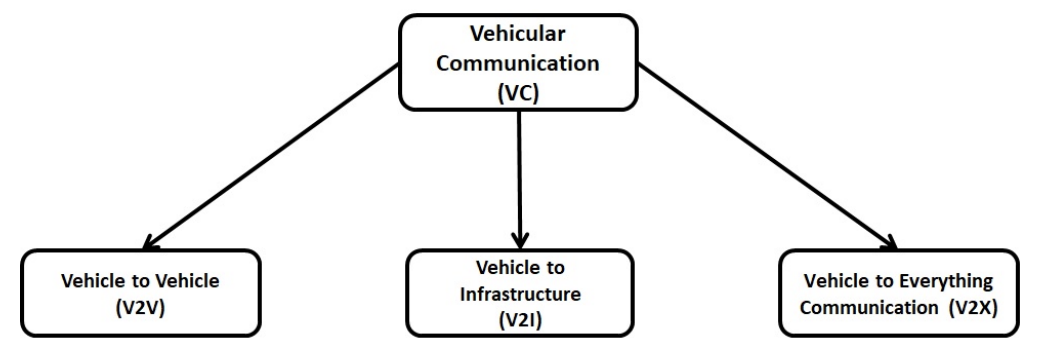
\includegraphics[width=0.7\linewidth]{figures/communication}
    \caption{VANETs}
    \label{fig:communication}
\end{figure}

\paragraph{Can BUS}
qualcosa  sul can bus per differenziare le comunicazioni interne  da quelle esterne presenntate sopra.

\subsubsection{Perception}\label{subsubsec:perception}
It is fundamental in AVs to perceive the environment and understand the context in which the vehicle is operating for obvious reasons.
The perception system is responsible for collecting data from various sensors, such as cameras, LiDAR, radar, and ultrasonic sensors, to create a detailed representation of the vehicle's surroundings.
In this case, it is important to consider the possible tempering that can be done on this sensor to alterate the perception of the vehicle, leading to dangerous situations \cite{kim2020cybersecurity, sec-sensors-2023, metro2020analysis, attacks-2020} .

Some of the main sensors used in AVs are:
\begin{enumerate}
    \item \textbf{Cameras}: Cameras are used to capture visual data, such as images and videos, of the vehicle's surroundings.
    \item \textbf{LiDAR (Light Detection and Ranging)}: LiDAR sensors use laser light to measure distances and create detailed 3D maps of the environment.
    \item \textbf{Radar (Radio Detection and Ranging)}: Radar sensors use radio waves to detect objects and measure their distance, speed, and direction.
    \item \textbf{Ultrasonic Sensors}: Ultrasonic sensors use sound waves to detect objects and measure their distance.
    \item \textbf{GPS (Global Positioning System)}: GPS sensors use satellite signals to determine the vehicle's location and navigate to a destination.
    \item \textbf{IMU (Inertial Measurement Unit)}: IMU sensors measure the vehicle's acceleration, orientation, and angular velocity.
\end{enumerate}

\begin{figure}[!htb]
    \centering
    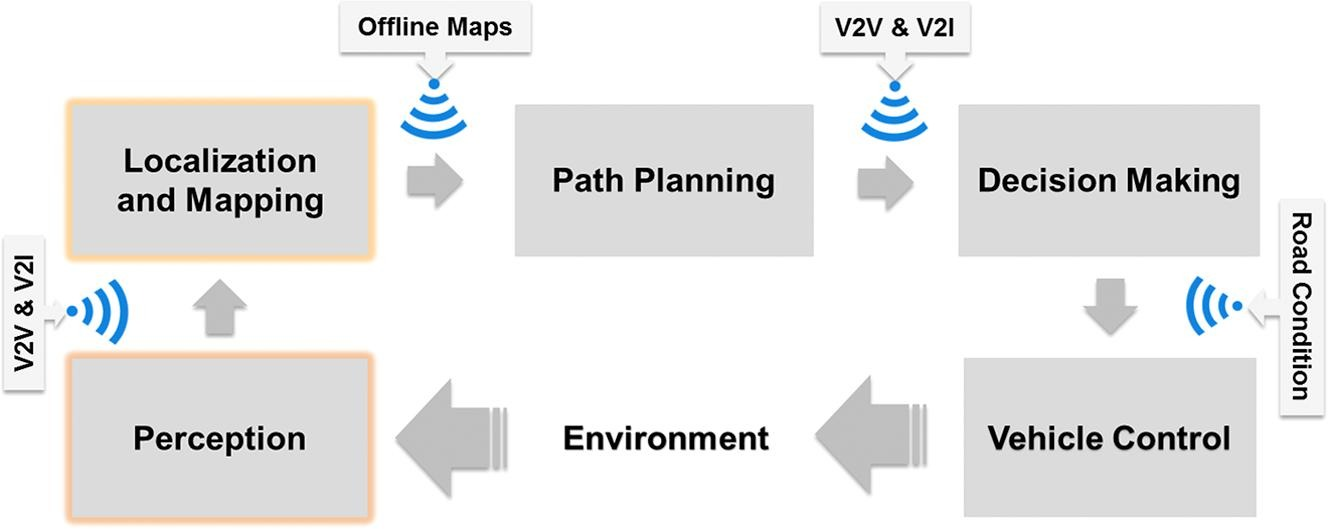
\includegraphics[width=0.7\linewidth]{figures/perception}
    \caption{Main sensors used in AVs}
    \label{fig:sensors}
\end{figure}

These sensors provide the critical data needed for navigation, obstacle
detection, and decision-making processes and are essential for ensuring the safety.
A tempering of these sensors can lead to dangerous situations \cite{unknown2020connected,cybersec} .

TODO In the next sections LINK A CYBERTREATS there will be a deep dive into the main sensors used in AVs and their vulnerabilities.


\subsection{Motivation}\label{subsec:motivation}

The motivation behind this survey is to provide a comprehensive overview of the current state of research on cybersecurity in autonomous vehicles.
The discussion begins with a brief history of autonomous vehicles (AVs) and an overview of some major attacks.
These incidents highlighted the importance of security in AV systems.
As a result, both manufacturers and researchers recognized the need to strengthen security measures.
This realization led to an emphasis on improving security by design.

There are some proposals like \cite{adu-kyere2023self-aware} that propose a self-aware security framework for AVs, and some standards like \cite{comparison-standard} that are trying to regulate the security of these systems, from the design to the deployment.
The problem is that the security of AVs is a complex issue to be solved by a single solution and without the collaboration of all the stakeholders.

The increasing introduction of new technologies in the automotive sector complicates the security of these systems.
Maintaining a high level of security becomes increasingly challenging without implementing a by-design approach.
The goal is to provide a holistic vision of the main threats and the current solutions on which the researchers are focusing on the cybersecurity field analysing main sensors and external connections with their vulnerabilities.


\subsection{Cyber-insecurity consequences}\label{subsec:cyber-insecurity}

Before introducing new threats of new autonomous vehicle technologies, it is important to understand some historical key attacks.
In the past, researchers have demonstrated various attacks on AVs, including remote hijacking, sensor spoofing, and data breaches.
The attack surface of AVs is expanding due to the increasing complexity of these systems, which rely on a combination of hardware, software, and communication technologies\cite{cybersec}.
This expansion is due to the aggressive attempts of manufacturers to
make vehicles fully autonomous in a short period of time and without considering the security implications.
This implied a lot of new technologies and new communication protocols keeping the focus always on the functionalities offered to the driver in terms of comfort.
The security of the vehicle has been considered as a secondary aspect, leading to a lot of vulnerabilities that can be exploited by attackers.

Some famous attacks that bring the attention to the security of AVs are:
\begin{enumerate}
    \item The Jeep Cherokee hack in 2015, where researchers remotely hijacked a Jeep Cherokee through its infotainment system, demonstrating the potential risks of cyber-attacks on connected vehicles \cite{miller2015remote} .
    \item The Tesla Model S hack in 2016, where researchers exploited vulnerabilities in the vehicle's software to take control of the car's brakes, door locks, and other critical systems \cite{tesla_hack}.
    \item The Nissan Leaf hack in 2016, where researchers demonstrated how an attacker could remotely control the vehicle's heating and air conditioning systems, drain the battery, and access the driver's personal information.
    \item The VW group hacked in 2016, where researchers discovered vulnerabilities in the keyless entry systems of several VW group vehicles, allowing attackers to unlock the doors and start the engine without the key fob \cite{garcia2016lock}.
\end{enumerate}

These are only some examples of the potential risks associated with AVs and the need for robust cybersecurity measures to protect against cyber-attacks.
One of the latest is the Tesla cybertruck vulnerabilities that have and continue to be exploited by attackers to gain access to the vehicle's systems and control its functions remotely.

\subsection{Social implications}\label{subsec:social-implications}

This section aims to provide a little insight into the social implications of autonomous vehicles.
The introduction of autonomous vehicles (AVs) is expected to have a profound impact on society \cite{thomas2020perception}, transforming transportation systems \cite{intelligent_transportation_2023}
, urban planning\cite{impact_autonomous_vehicles_2018}, and the economy~\cite{economic_aspects_2020}.

\begin{table}[ht]
    \centering
    \begin{tabular}{|l|l|}
        \hline
        \textbf{Advantages} & \textbf{Disadvantages} \\ \hline
        Casualty: AVs can significantly reduce the number of accidents. & Law: The definition of legal responsibilities can hinder the implementation of AVs. \\ \hline
        Fewer Expenses: Precise autonomous driving can reduce fuel consumption and increase the conservation of other parts. & Threat: AVs can be more vulnerable to network hacks because of the present computer-controlled functions. \\ \hline
        Productivity: The journey can be productive by performing other activities than driving. & Employment: There will be many job losses due to AVs in the transportation sector. \\ \hline
        Comfort: Interiors of AVs can be comfortable and spacious. & Price: The price of AVs is initially high, but after greater adoption, the price is going to decrease. \\ \hline
    \end{tabular}
    \caption{Advantages and Disadvantages of Autonomous Vehicles (AVs) from \cite{ahangar2021survey} }\label{tab:table}
\end{table}

